\subsection{Opacity measurement consistency tests}

{\bf copy from the 'Instru' paper}

\begin{figure}
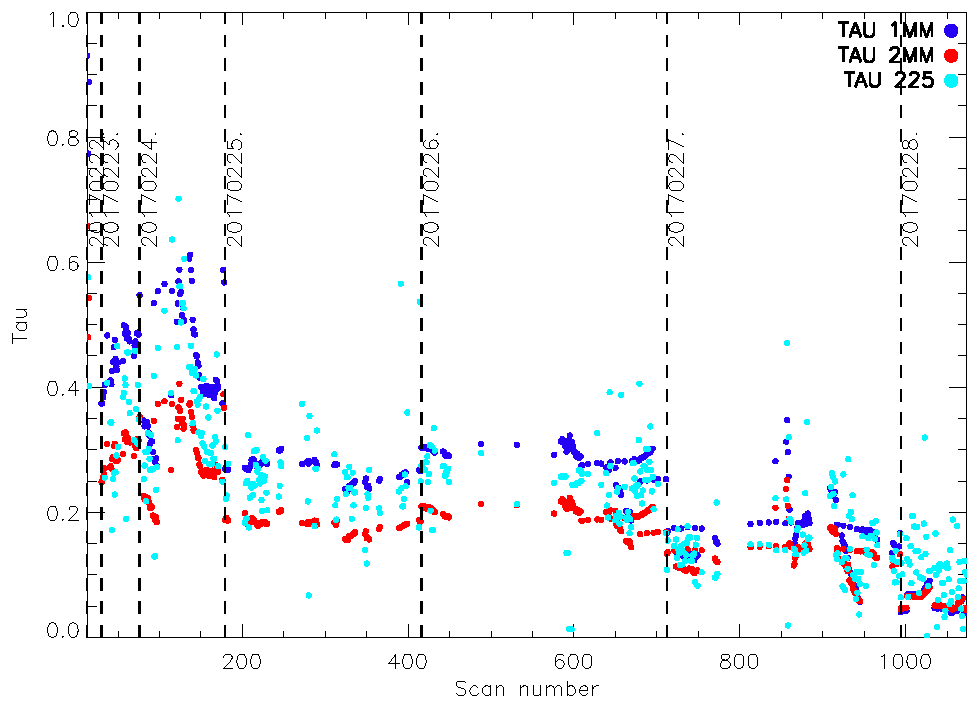
\includegraphics[scale=0.75]{../../Paper_NIKA2_Technical/opacity_evol_run22.pdf}
\caption{Atmospheric opacity as measured from the IRAM 225\,GHz taumeter (cyan), and from the NIKA2 data at 150 (red) and 260\,GHz (blue) during the February 2017 NIKA2 commissioning campaign. We stress the fact that the IRAM 225\,GHz taumeter data is not used for the atmospheric correction and is plotted here just for comparison.
  \label{fig:taumeas}}
\end{figure}

We observe that the skydip-fitted $\tau$ values are, as expected,
common between different detectors of the same array. By comparing
the results of different skydips, we have verified experimentally
that the coefficients $C_0$, $C_1$ are stable, within the fit
errors, on very long time scales within a cooldown cycle. The
coefficients can thus be applied to the whole observing campaign
in order to recover the opacity of each scan.

In Fig.~\ref{fig:taumeas} we present the evolution of the NIKA2 in-band opacities for several
scans of the commissioning run held in February 2017. These are
compared to the IRAM tau-meter lectures. We observe a global
trend agreement between the IRAM tau-meter suggested opacity
(225 GHz) and the NIKA2 values. These latter show, however,
a smaller dispersion. We find an average ratio between the
150 GHz and the 260 GHz NIKA2 derived opacities of about
0.6, consistent with model expectations. We notice however that
the 150 GHz-to-260 GHz opacity ratio varies significantly for
opacities (at 150 GHz) below 0.2. This effect is likely to be
linked to an $O_2$ atmospheric line which becomes saturated. This
point is, however, still under investigation.


